\documentclass{article}

\usepackage[english]{babel}
\usepackage{float}
\usepackage[letterpaper,top=2cm,bottom=2cm,left=3cm,right=3cm,marginparwidth=2cm]{geometry}
\usepackage{amsmath}
\usepackage{amssymb}
\usepackage{graphicx}
\usepackage{grffile}
\usepackage{booktabs}
\usepackage{array}
\usepackage{tabularx}
\usepackage{caption}
\usepackage{verbatim}
\captionsetup[figure]{justification=centering}
\usepackage[colorlinks=true, allcolors=blue]{hyperref}
\setlength{\emergencystretch}{3em}

\title{\textbf{ME 144L Pre-Lab 9: PMDC Motor Modeling, Drives, and Sensing}}
\author{Alejandro Diaz \\ TA: Gabrielle Naquila}
\date{April 6, 2026}

\begin{document}
\maketitle

% ============================================================
\section{PMDC Motor Circuit Schematic}
% ============================================================

\begin{figure}[H]
    \centering
    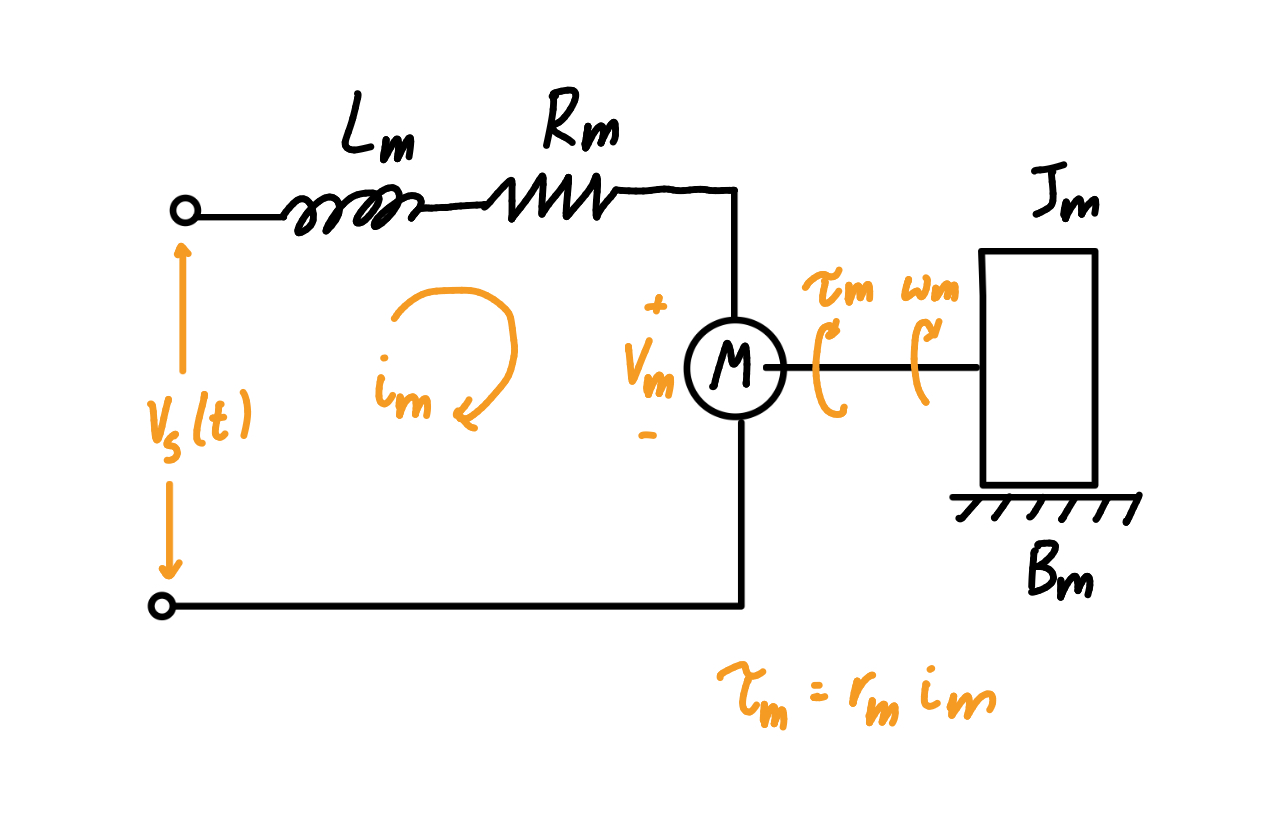
\includegraphics[width=0.6\linewidth]{figures/circuit_schematic.jpg}
    \caption{PMDC motor circuit schematic showing connections, resistance, and back-EMF source.}
    \label{fig:circuit_schematic}
\end{figure}

\noindent To estimate the three key steady-state PMDC motor model parameters ($R_m$, $r_m$, $B_m$), the following measurements can be made during testing:

\begin{table}[H]
    \centering
    \caption{Required measurements for PMDC motor parameter estimation.}
    \label{tab:measurements}
    \begin{tabular}{lll}
        \toprule
        \textbf{Measurement} & \textbf{Symbol} & \textbf{Physical Meaning} \\
        \midrule
        Terminal resistance   & $R_m$       & Resistance of the armature winding, measured \\
                              &             & directly across the motor terminals with an ohmmeter \\
        \addlinespace
        Input voltage         & $V_{in}$    & Voltage applied to motor; set by PWM duty cycle \\
        \addlinespace
        Motor current         & $i_m$       & Armature current measured with a DMM in series \\
                              &             & or from sensing resistor \\
        \addlinespace
        Shaft speed           & $\omega_m$  & Steady-state rotor speed read from the magnetic \\
                              &             & encoder on the motor shaft. \\
        \addlinespace
        Calculated back-EMF   & $V_m$       & Voltage computed as $V_m = V_{in} - R_m\, i_m$ \\
        \bottomrule
    \end{tabular}
\end{table}

\noindent At each PWM level, $V_{in}$, $\omega_m$, and $i_m$ are recorded at steady state, with $V_m = V_{in} - R_m i_m$ calculated from each row. From this data, $r_m$ and $B_m$ can be determined, and $R_m$ is measured with an ohmmeter at the motor terminals.

% ============================================================
\section{Estimating the Motor Constant ($r_m$)}
% ============================================================

The motor constant $r_m$ (N$\cdot$m/A) relates the electromagnetic torque to the armature current. Additionally, it relates the back-EMF voltage to the shaft speed. The power conversion is written as:

\begin{equation}
    P_{\text{electrical}} = V_m\, i_m = \tau_m\, \omega_m = P_{\text{mechanical}}
    \label{eq:power_balance}
\end{equation}

\noindent Using the gyrator operator, the relation for motor torque and voltage are:

\begin{align}
    \tau_m &= r_m\, i_m \label{eq:torque_const} \\
    V_m    &= r_m\, \omega_m \label{eq:backemf_const}
\end{align}

\noindent The back-EMF relation $V_m = r_m \omega_m$ is not measured directly but is calculated from the measured speed and known armature resistance:

\begin{equation}
    V_m = V_{in} - R_m\, i_m
    \label{eq:backemf_calc}
\end{equation}

\noindent The motor is run across a range of PWM duty cycles, and at each operating point, the input voltage $V_{in}$, shaft speed $\omega_m$, and motor current $i_m$ are recorded. From each data point, the back-EMF is calculated from the equation shown above. The slope of a linear fit is used to solve for $r_m$:

\begin{equation}
    r_m = \frac{\Delta V_m}{\Delta \omega_m}
    \label{eq:rm_regression}
\end{equation}

\noindent The main assumption is that the motor is operating at steady state so that the inductive voltage drop is zero and the full voltage difference appears as back-EMF. under this assumption, the relationship is inherently linear for the PMDC motor.

% ===========================================================
\section{Torque-Speed Curve and Loss Torque Coefficient}
% ===========================================================

The steady-state torque-speed curve is derived by considering resistance $R_m$ and rotational friction $B_m$), as shown in the equation below.

\begin{equation}
    \tau_m = r_m\, i_m = \frac{r_m}{R_m}\left(V_{in} - V_m\right)
    \label{eq:ideal_torque}
\end{equation}

\noindent Where $V_m$ is the back-EMF. For linear viscous friction, the output torque delivered to an external load without gear train losses is:

\begin{equation}
    \tau_o = \frac{r_m}{R_m}\left(V_{in} - r_m\, \omega_m\right) - B_m\, \omega_m
    \label{eq:torque_intermediate}
\end{equation}

\noindent Expanding and rearranging terms gives the final torque-speed relation:

\begin{equation}
    \;\tau_o = \frac{r_m}{R_m}\, V_{in} - \left(\frac{r_m^2}{R_m} + B_m\right) \omega_m\;
    \label{eq:torque_speed}
\end{equation}

\noindent This relation is linear in $\omega_m$, with slope $\left(r_m^2/R_m + B_m\right)$ capturing electrical and mechanical losses. At $\omega_m = 0$ the motor produces maximum (stall) torque $\tau_s = (r_m/R_m)\,V_{in}$; at $\tau_o = 0$ it reaches no-load speed. Increasing $V_{in}$ shifts the curve upward, producing parallel lines at each PWM level. With no external load, all motor torque goes into friction, so at steady state $\tau_m = r_m\, i_m = B_m\, \omega_m$. Plotting $r_m\, i_m$ versus $\omega_m$ across the no-load data and fitting a line gives $B_m$ as the slope.

% ============================================================
\section{SparkFun TB6612FNG Library Installation}
% ============================================================

Sparkfun TB6612FNG library has been successfully installed in the Arduino IDE, and returns the \texttt{\#include <SparkFun\_TB6612.h>} header without errors.

\end{document}
